% NeST Policy 3: convolutional feature-map growth (single-card figure).
\documentclass[tikz,border=8pt]{standalone}
\usepackage{amsmath,amssymb,bm}
\usetikzlibrary{positioning,calc}
\begin{document}
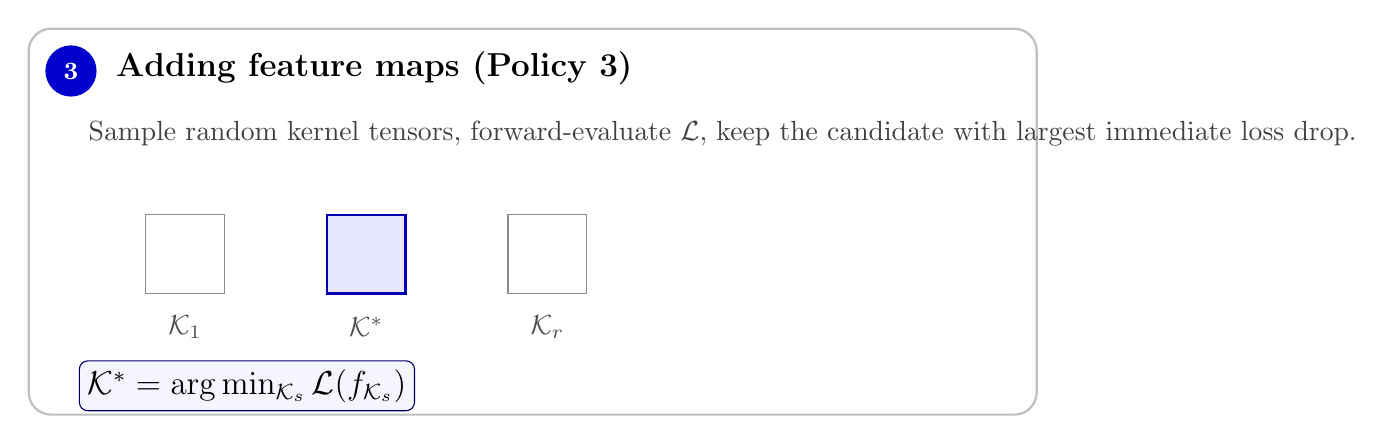
\begin{tikzpicture}[font=\sffamily]
\tikzset{
  card/.style={draw=black!25, rounded corners=8pt, fill=white, line width=0.8pt},
  chip/.style={draw=blue!40!black, rounded corners=3pt, fill=blue!4, inner sep=3pt},
  stepnode/.style={circle, fill=blue!80!black, text=white, minimum size=6.5mm, inner sep=0pt, font=\bfseries\small}
}
\node[card, minimum width=12.8cm, minimum height=4.9cm, anchor=north west] (c) at (0,0) {};
\node[stepnode] at ($(c.north west)+(0.55,-0.55)$) {3};
\node[anchor=west, font=\bfseries\large] at ($(c.north west)+(1.0,-0.52)$) {Adding feature maps (Policy~3)};
\node[anchor=west, font=\normalsize, text=black!75] at ($(c.north west)+(0.65,-1.35)$)
  {Sample random kernel tensors, forward-evaluate $\mathcal{L}$, keep the candidate with largest immediate loss drop.};
\node[draw=black!45, minimum width=1.0cm, minimum height=1.0cm] (k1) at ($(c.south west)+(2.0,2.05)$) {};
\node[draw=blue!70!black, fill=blue!10, line width=0.9pt, minimum width=1.0cm, minimum height=1.0cm] (k2) at ($(c.south west)+(4.3,2.05)$) {};
\node[draw=black!45, minimum width=1.0cm, minimum height=1.0cm] (k3) at ($(c.south west)+(6.6,2.05)$) {};
\node[font=\normalsize, text=black!70] at ($(k1)+(0,-0.92)$) {$\mathcal{K}_1$};
\node[font=\normalsize, text=black!70] at ($(k2)+(0,-0.92)$) {$\mathcal{K}^\ast$};
\node[font=\normalsize, text=black!70] at ($(k3)+(0,-0.92)$) {$\mathcal{K}_r$};
\node[chip, anchor=west, font=\large] at ($(c.south west)+(0.65,0.38)$)
{$\mathcal{K}^\ast=\arg\min_{\mathcal{K}_s}\mathcal{L}\!\left(f_{\mathcal{K}_s}\right)$};
\end{tikzpicture}
\end{document}
